\chapter{Result}
\label{chp:result}
\section{Overview}
\label{result:overview}

This chapter presents the results of comprehensive evaluations conducted to assess the performance and suitability of the proposed FlatCitybuf format against existing CityJSON encoding approaches. The evaluation followed three complementary methodologies to provide a holistic understanding of the format's capabilities.

The assessment framework employed three distinct methodological approaches. First, file size comparison was conducted to evaluate storage efficiency across different datasets and encoding formats.

Second, performance benchmarks were conducted on a laptop environment to evaluate the computational efficiency of the encoding format. These benchmarks measured read operation time for files of varying sizes, memory consumption during processing operations, and storage efficiency through file size comparisons. The benchmark utilised the datasets from \citet{ledoux_2024} and additional datasets from PLATEAU, providing direct comparability with previous studies on CityJSON and CityJSONSeq formats. All operations were conducted multiple times to ensure statistical reliability, with warm-up iterations to eliminate caching effects.

Third, to assess real-world application performance in web environments, browser-based benchmarks were conducted to measure the time required to fetch subsets of data. These tests focused on evaluating how efficiently the format enables selective data retrieval through HTTP Range requests, allowing clients to access only the specific portions of data they need rather than downloading entire datasets. This approach provides insights into the practical benefits of the format for web-based applications where bandwidth optimization and response time are critical factors.

The following sections present detailed results from each evaluation approach, followed by integrated analyses that synthesise findings across methodologies to provide comprehensive insights into the performance characteristics of the FlatCitybuf format.

\section{File Size Comparison}
\label{result:file_size_comparison}

\subsubsection{Datasets}
\label{result:overview:dataset}
To evaluate file sizes and conduct both local and web-based benchmarks, we employed a diverse range of datasets from \citet{ledoux_2024} supplemented with additional datasets from PLATEAU. Comprehensive information regarding these datasets and their attributions is provided in \autoref{appendix:dataset}.

\subsection{File size results}
\label{result:overview:filesize_comparison}

\autoref{tab:dataset_comparison} presents a comparison of datasets in both CityJSONSeq and FlatCityBuf formats. The results demonstrate that FlatCityBuf encoding achieves superior compression for several datasets, including Helsinki, Ingolstadt, and New York City, with compression factors of 16.36\%, 19.09\%, and 20.17\% respectively. Conversely, the PLATEAU datasets exhibit the opposite trend, with CityJSONSeq format demonstrating better storage efficiency.

\todo{Add whole 3DBAG}
\begin{table*}
  \centering
  \begin{threeparttable}
    \caption{The datasets used for the benchmark.}
    \label{tab:dataset_comparison}
    \scriptsize
    \setlength{\tabcolsep}{4pt}
    \begin{tabular}{@{}lrrlrrr@{\hskip 3pt}rrrr@{}}
      \toprule
      & \multicolumn{3}{c}{\textbf{dataset}} & \multicolumn{3}{c}{\textbf{size of file}} & \multicolumn{4}{c}{\textbf{attributes}} \\
      \cmidrule(lr){2-4} \cmidrule(lr){5-7} \cmidrule(lr){8-11}
      & CityObj & CityFeat & app.$^{\text{(a)}}$ & CityJSONSeq & FlatCityBuf & compr.$^{\text{(b)}}$ & verts & avg$^{\text{(c)}}$ & obj$^{\text{(d)}}$ & sem$^{\text{(e)}}$ \\
      \midrule
      \textbf{3DBAG}          & 2221    & 1110   &      & \qty{5.87}{\mega\byte}  & \qty{6.23}{\mega\byte}  & $-6.02\%$  & 82612    & 74.43    & 37 & 1 \\
      \textbf{3DBV}           & 71634   & 71634  &      & \qty{317.34}{\mega\byte}& \qty{280.92}{\mega\byte}& $11.48\%$  & 4992893  & 69.70    & 64 & 0 \\
      \textbf{Helsinki}       & 77267   & 77231  &      & \qty{412.44}{\mega\byte}& \qty{344.96}{\mega\byte}& $16.36\%$  & 3039107  & 39.35    & 27 & 9 \\
      \textbf{Helsinki\_tex}  & 77267   & 77231  & tex  & \qty{643.70}{\mega\byte}& \qty{545.29}{\mega\byte}& $15.29\%$  & 3039107  & 39.35    & 28 & 9 \\
      \textbf{Ingolstadt}     & 379     & 55     &      & \qty{3.84}{\mega\byte}  & \qty{3.11}{\mega\byte}  & $19.09\%$  & 88001    & 1600.02  & 33 & 13 \\
      \textbf{Montréal}       & 294     & 294    & tex  & \qty{4.60}{\mega\byte}  & \qty{4.80}{\mega\byte}  & $-4.38\%$  & 32242    & 109.67   & 0  & 0 \\
      \textbf{NYC}            & 23777   & 23777  &      & \qty{95.45}{\mega\byte} & \qty{76.20}{\mega\byte} & $20.17\%$  & 1044145  & 43.91    & 3  & 3 \\
      \textbf{Railway}        & 121     & 38     & tex+mat  & \qty{4.05}{\mega\byte}  & \qty{3.75}{\mega\byte}  & $7.35\%$   & 73856    & 1943.58  & 3  & 0 \\
      \textbf{Rotterdam}      & 853     & 853    & tex  & \qty{2.69}{\mega\byte}  & \qty{2.80}{\mega\byte}  & $-3.98\%$  & 26679    & 31.28    & 5  & 0 \\
      \textbf{Vienna}         & 1322    & 307    &      & \qty{4.81}{\mega\byte}  & \qty{4.12}{\mega\byte}  & $14.32\%$  & 47229    & 153.84   & 7  & 4 \\
      \textbf{Zürich}         & 198699  & 52834  &      & \qty{247.12}{\mega\byte}& \qty{188.63}{\mega\byte}& $23.67\%$  & 3564542  & 67.47    & 8  & 0 \\
      \textbf{PLATEAU\_bldg}  & 10405   & 4307   &      & \qty{76.94}{\mega\byte} & \qty{79.41}{\mega\byte} & $-3.22\%$  & 147754   & 34.31    & 14 & 2 \\
      \textbf{PLATEAU\_brid}  & 60      & 8      &      & \qty{4.78}{\mega\byte}  & \qty{5.21}{\mega\byte}  & $-9.09\%$  & 16357    & 2044.62  & 5  & 2 \\
      \textbf{PLATEAU\_rwy}   & 412     & 412    &      & \qty{4.15}{\mega\byte}  & \qty{4.23}{\mega\byte}  & $-1.90\%$  & 5846     & 14.19    & 3  & 2 \\
      \textbf{PLATEAU\_tran}  & 8136    & 8136   &      & \qty{26.47}{\mega\byte} & \qty{26.62}{\mega\byte} & $-0.54\%$  & 45992    & 5.65     & 3  & 2 \\
      \textbf{PLATEAU\_tun}   & 21      & 3      &      & \qty{4.86}{\mega\byte}  & \qty{4.64}{\mega\byte}  & $4.41\%$   & 12306    & 4102.00  & 4  & 1 \\
      \textbf{PLATEAU\_veg}   & 936     & 936    &      & \qty{1.78}{\mega\byte}  & \qty{2.32}{\mega\byte}  & $-30.50\%$ & 2567     & 2.74     & 3  & 0 \\
      \textbf{Tokyo\_PLATEAU} & 49764   & 38627  &      & \qty{209.62}{\mega\byte}& \qty{216.76}{\mega\byte}& $-3.41\%$  & 316607   & 8.20     & 15 & 1 \\
      \bottomrule
    \end{tabular}
    \begin{tablenotes}[flushleft]
      \footnotesize
    \item[a] appearance: `tex' indicates textures are stored; `mat' indicates materials are stored
    \item[b] compression factor is $\frac{\text{CityJSONSeq} - \text{FlatCityBuf}}{\text{CityJSONSeq}}$ (positive values indicate size reduction)
    \item[c] average number of vertices per feature
    \item[d] number of attributes in city objects
    \item[e] number of semantic surface attributes in city objects
    \end{tablenotes}
  \end{threeparttable}
\end{table*}

\subsection{Analysis of file size results}
\label{result:overview:analysis_of_file_size_results}
Although \autoref{result:overview:filesize_comparison} provides a summary of file size comparisons, the factors influencing these outcomes require further investigation. This section analyses the underlying causes through controlled experiments with simplified datasets.

\subsubsection{Level of detail}
\label{result:overview:analysis_of_file_size_results:level_of_detail}

To examine how level of detail (LOD) affects file size, we conducted a series of tests using the TU Delft BK building model at various LOD levels. Each LOD variant was systematically extracted from the original model, with attributes and semantic information deliberately removed to isolate the effect of geometric complexity. \autoref{tab:lod_comparison} presents the results of this analysis.

Since each test dataset contains only a single city feature, we compare feature sizes rather than total file sizes. This approach is necessary because FlatCityBuf incorporates a larger header structure, which would disproportionately affect comparisons involving minimal features.

The results demonstrate that while file sizes increase with higher levels of detail, the compression factor remains largely independent of LOD. Both formats show similar proportional growth in size as geometric complexity increases, with FlatCityBuf consistently achieving approximately 24-25\% size reduction compared to CityJSONSeq regardless of the LOD level. This suggests that the compression efficiency is determined by the underlying format design rather than the geometric complexity of the data.

\begin{table}[htbp]
  \centering
  \caption{Comparison of file sizes across different levels of detail for the TU Delft BK building model.}
  \label{tab:lod_comparison}
  \begin{tabular}{@{}lrrrr@{}}
    \toprule
    \textbf{Dataset} & \textbf{FlatCityBuf}$^{\text{(a)}}$ & \textbf{CityJSONSeq}$^{\text{(b)}}$ & \textbf{Compression} & \textbf{Vertices} \\
    \midrule
    TUD BK All & \qty{139.75}{\kilo\byte} & \qty{189.01}{\kilo\byte} & $26.08\%$ & 4549 \\
    TUD BK LOD0 & \qty{12.77}{\kilo\byte} & \qty{20.72}{\kilo\byte} & $38.11\%$ & 785 \\
    TUD BK LOD1.2 & \qty{37.45}{\kilo\byte} & \qty{49.40}{\kilo\byte} & $24.23\%$ & 1350 \\
    TUD BK LOD1.3 & \qty{44.66}{\kilo\byte} & \qty{59.25}{\kilo\byte} & $24.67\%$ & 1600 \\
    TUD BK LOD2.2 & \qty{62.02} {\kilo\byte} & \qty{82.74}{\kilo\byte} & $25.07\%$ & 2168 \\
    \bottomrule
  \end{tabular}
  \begin{tablenotes}[flushleft]
    \footnotesize
  \item[a] Average feature size in bytes in FlatCityBuf: $\frac{\text{Total FlatCityBuf size}}{\text{Number of features}}$
  \item[b] Average feature size in bytes in CityJSONSeq: $\frac{\text{Total CityJSONSeq size}}{\text{Number of features}}$

  \end{tablenotes}
\end{table}

\subsubsection{Attributes}
\label{result:overview:analysis_of_file_size_results:attributes}

To assess the impact of attributes on file size, we tested simple cube models from \citep{cityjson_dataset} with varying numbers of attributes. We systematically generated random attributes for each test case, examining both integer and string data types to determine their effect on compression efficiency. \autoref{tab:attribute_comparison} presents the results of this analysis.

\begin{table}[htbp]
  \centering
  \caption{Comparison of file sizes with varying numbers of attributes for simple cube models.}
  \label{tab:attribute_comparison}
  \begin{tabular}{@{}lrrrr@{}}
    \toprule
    \textbf{Dataset} & \textbf{FlatCityBuf}$^{\text{(a)}}$ & \textbf{CityJSONSeq}$^{\text{(b)}}$ & \textbf{Compression} & \textbf{Attributes} \\
    \midrule
    10 attributes (int) & \qty{580}{\byte} & \qty{611}{\byte} & $5.07\%$ & 10 \\
    100 attributes (int) & \qty{1.62}{\kilo\byte} & \qty{2.44}{\kilo\byte} & $33.65\%$ & 100 \\
    1000 attributes (int) & \qty{12.17}{\kilo\byte} & \qty{21.78}{\kilo\byte} & $44.13\%$ & 1000 \\
    10 attributes (string) & \qty{580}{\byte} & \qty{611}{\byte} & $5.07\%$ & 10 \\
    100 attributes (string) & \qty{1.62}{\kilo\byte} & \qty{2.44}{\kilo\byte} & $33.65\%$ & 100 \\
    1000 attributes (string) & \qty{12.17}{\kilo\byte} & \qty{21.78}{\kilo\byte} & $44.13\%$ & 1000 \\
    \bottomrule
  \end{tabular}
  \begin{tablenotes}[flushleft]
    \footnotesize
  \item[a] Average feature size in bytes in FlatCityBuf: $\frac{\text{Total FlatCityBuf size}}{\text{Number of features}}$
  \item[b] Average feature size in bytes in CityJSONSeq: $\frac{\text{Total CityJSONSeq size}}{\text{Number of features}}$
  \end{tablenotes}
\end{table}

The randomly generated attributes in our test datasets followed a consistent pattern, as shown in the example below:

\begin{verbatim}
{
  "type": "Building",
  "geometry": [...],
  "attributes": {
    "attr_1": "value_1",
    "attr_2": "value_2",
    "attr_3": "value_3",
    "attr_4": "value_4",
    "attr_5": "value_5",
    ...
    "attr_n": "value_n"
  }
}
\end{verbatim}

For integer attribute tests, all values were randomly generated integers between 0 and 1000. For string attribute tests, values were randomly generated strings of varying lengths between 5 and 15 characters. This approach ensured a realistic representation of typical attribute data while maintaining controlled test conditions.

\begin{figure}[htbp]
  \centering
  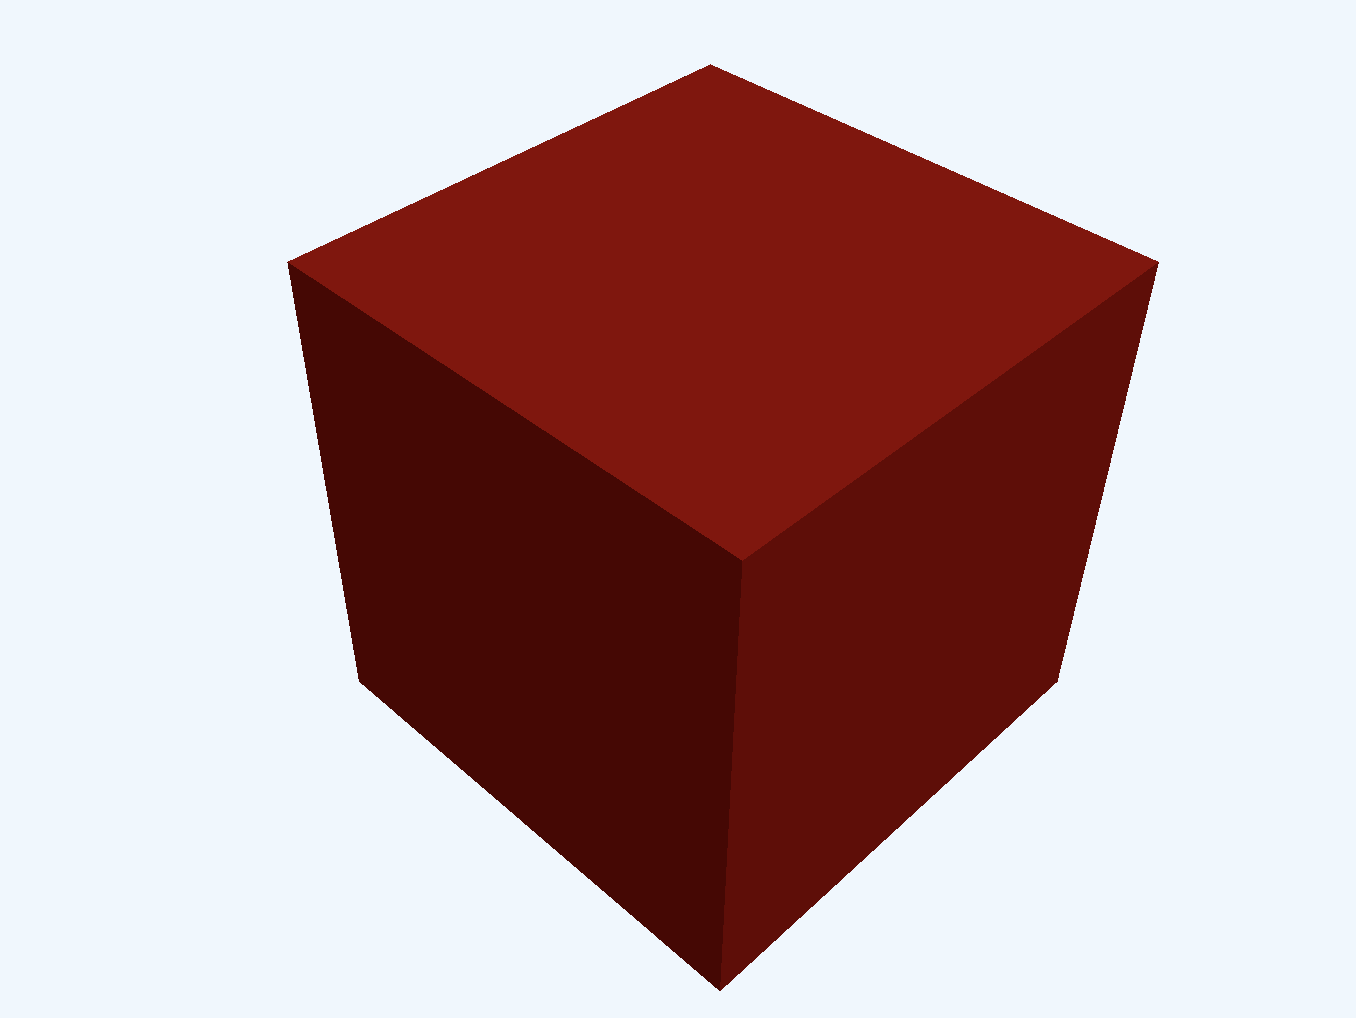
\includegraphics[width=0.48\textwidth]{figs/result_analysis/cube.png}
  \caption{Simple cube model used for attribute testing. This basic geometric structure provides a controlled environment for evaluating the impact of attributes on file size.}
  \label{fig:simple_cube}
\end{figure}

The results reveal a clear pattern: FlatCityBuf's compression advantage over CityJSONSeq increases substantially with the number of attributes. With only 10 attributes, the compression benefit is minimal at 5.07\%, but rises markedly to 33.65\% with 100 attributes and reaches 44.13\% with 1000 attributes.

This efficiency stems from FlatCityBuf's architectural design, which stores the attribute schema once in the file header. Each feature subsequently references attributes using only a 2-byte (u16) index, while CityJSONSeq must replicate identical attribute keys across all features. Although additional attributes increase the header size, this overhead is distributed across all features in the dataset. The header remains relatively compact—even with 1000 attributes, it occupies only a few tens of kilobytes.

These characteristics render FlatCityBuf particularly advantageous for datasets containing numerous attributes. The same efficiency applies to semantic surface attributes, where the schema-based approach provides similar compression benefits when features contain multiple surfaces with rich semantic information.

\subsubsection{Geometry complexity}
\label{result:overview:analysis_of_file_size_results:geometric_complexity}

To evaluate how geometric complexity influences file size, we analysed models with varying numbers of vertices. The test utilised two geometrically distinct models from the TU Delft campus dataset—one simple and one complex. To isolate the effect of geometry, attributes and semantic information were removed, leaving only the essential geometric components required by CityJSON. \autoref{tab:geometry_comparison} presents the numerical results of this analysis, while \autoref{fig:geometry_comparison} provides visual comparisons of the models.

\begin{table}[htbp]
  \centering
  \caption{Comparison of file sizes with varying geometric complexity.}
  \label{tab:geometry_comparison}
  \begin{tabular}{@{}lrrrr@{}}
    \toprule
    \textbf{Dataset} & \textbf{FlatCityBuf}$^{\text{(a)}}$ & \textbf{CityJSONSeq}$^{\text{(b)}}$ & \textbf{Compression} & \textbf{Vertices/Feature} \\
    \midrule
    TUD BK & \qty{139.75}{\kilo\byte} & \qty{189.01}{\kilo\byte} & $26.06\%$ & 4549 \\
    TUD Simple & \qty{13.12}{\kilo\byte} & \qty{15.42}{\kilo\byte} & $14.94\%$ & 340 \\
    \bottomrule
  \end{tabular}
  \begin{tablenotes}[flushleft]
    \footnotesize
  \item[a] Average feature size in bytes in FlatCityBuf: $\frac{\text{Total FlatCityBuf size}}{\text{Number of features}}$
  \item[b] Average feature size in bytes in CityJSONSeq: $\frac{\text{Total CityJSONSeq size}}{\text{Number of features}}$
  \end{tablenotes}
\end{table}

\begin{figure}[htbp]
  \centering
  \begin{subfigure}{0.48\textwidth}
    \centering
    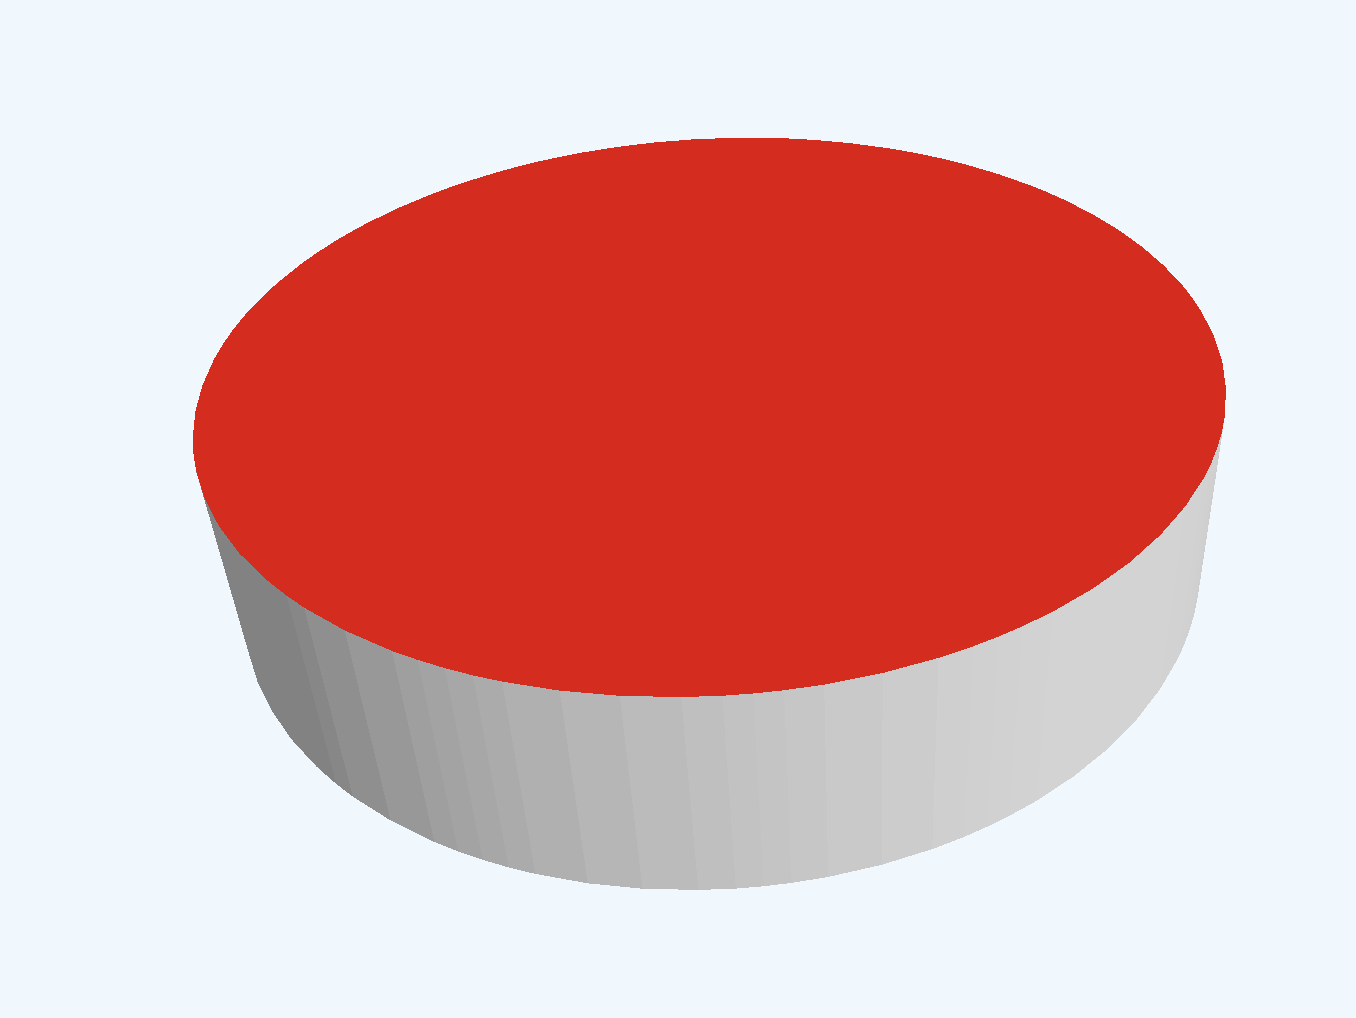
\includegraphics[width=\textwidth]{figs/result_analysis/tud_simple.png}
    \caption{TUD Simple model (340 vertices/feature)}
    \label{fig:tud_simple}
  \end{subfigure}
  \hfill
  \begin{subfigure}{0.48\textwidth}
    \centering
    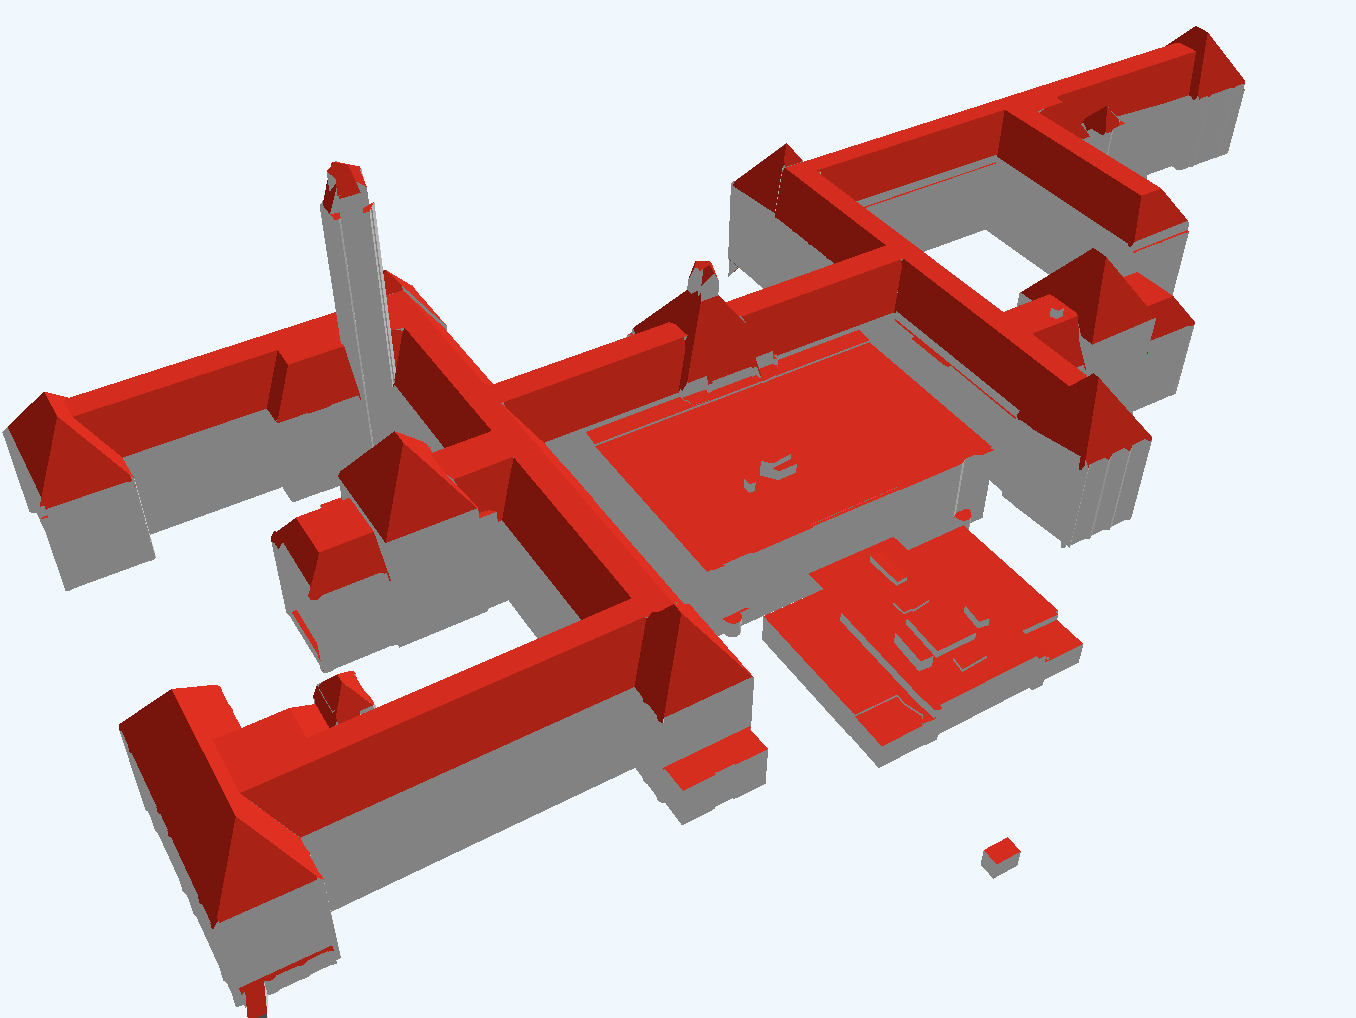
\includegraphics[width=\textwidth]{figs/result_analysis/tud_bk.png}
    \caption{TUD BK model (4549 vertices/feature)}
    \label{fig:tud_bk}
  \end{subfigure}
  \caption{Visual comparison of models with different geometric complexity.}
  \label{fig:geometry_comparison}
\end{figure}

The results demonstrate that geometric complexity significantly affects compression efficiency, with FlatCityBuf achieving better compression for more intricate models. The TU Delft BK building model, containing 4549 vertices per feature, exhibits a higher compression rate of 26.06\% compared to the simpler model with 340 vertices at 14.94\%.

This differential appears to result from the expanding boundary field as geometry becomes more complex. FlatCityBuf employs a strongly typed representation of boundaries (using u32 integers) that maintains a constant size for encoding each vertex, whereas CityJSONSeq requires additional bytes due to its text-based format. This fundamental difference in geometry encoding becomes increasingly advantageous for FlatCityBuf as geometric complexity rises.

\subsubsection{Vertices and coordinates}
\label{result:overview:analysis_of_file_size_results:vertices_and_coordinates}

To investigate how coordinate scale affects file size, we conducted tests using identical cube geometries with varying coordinate magnitudes. These models contain the same number of vertices (8 per feature) but differ in their coordinate scale values. \autoref{tab:vertices_comparison} presents the results of this analysis, utilising the same base models as in \autoref{result:overview:analysis_of_file_size_results:attributes}.

\begin{table}[htbp]
  \centering
  \caption{Comparison of file sizes with varying coordinate scales.}
  \label{tab:vertices_comparison}
  \begin{tabular}{@{}lrrrr@{}}
    \toprule
    \textbf{Dataset} & \textbf{FlatCityBuf}$^{\text{(a)}}$ & \textbf{CityJSONSeq}$^{\text{(b)}}$ & \textbf{Compression} & \textbf{Scale} \\
    \midrule
    Cube (1) & \qty{476}{\byte} & \qty{370}{\byte} & $-28.65\%$ & 1 \\
    Cube (10) & \qty{476}{\byte} & \qty{459}{\byte} & $-3.70\%$ & 10 \\
    Cube (1k) & \qty{476}{\byte} & \qty{507}{\byte} & $6.11\%$ & 1,000 \\
    Cube (1M) & \qty{476}{\byte} & \qty{579}{\byte} & $17.79\%$ & 1,000,000 \\
    \bottomrule
  \end{tabular}
  \begin{tablenotes}[flushleft]
    \footnotesize
  \item[a] Average feature size in bytes in FlatCityBuf: $\frac{\text{Total FlatCityBuf size}}{\text{Number of features}}$
  \item[b] Average feature size in bytes in CityJSONSeq: $\frac{\text{Total CityJSONSeq size}}{\text{Number of features}}$
  \end{tablenotes}
\end{table}

The results reveal an intriguing relationship between coordinate scale and file size in both formats. FlatCityBuf maintains a consistent size of 476 bytes regardless of coordinate magnitude, demonstrating its fixed-size binary encoding for numeric values. In contrast, CityJSONSeq's file size increases proportionally with larger coordinate values, growing from 370 bytes with single-digit coordinates to 579 bytes with million-scale coordinates.

This behaviour occurs because FlatCityBuf stores coordinates as fixed-size 32-bit integers, while CityJSONSeq, being a text-based format, requires more characters to represent larger numbers. Consequently, FlatCityBuf transitions from being less efficient than CityJSONSeq for small coordinate values (-28.65\%) to substantially more efficient for large coordinate values (17.79\%).

This characteristic explains the pattern observed in \autoref{result:overview:filesize_comparison}. FlatCityBuf demonstrates lower storage efficiency for PLATEAU datasets, likely because these datasets employ geographic coordinate systems with values typically between -180 and 180. Since CityJSON quantises coordinates through the \texttt{Transform} field, latitude and longitude values can be represented as relatively small integers. Conversely, datasets where FlatCityBuf performs better—such as NYC and Helsinki—use local coordinate systems (in metres) with larger internal values, resulting in improved compression efficiency with FlatCityBuf.

\subsubsection{Summary of File Size Analysis}
\label{result:overview:analysis_of_file_size_results:summary}

The comprehensive analysis of various factors affecting file size reveals distinct patterns in the compression performance of FlatCityBuf compared to CityJSONSeq:

\begin{itemize}
  \item \textbf{Level of Detail:} The analysis demonstrates that geometric detail levels have minimal impact on compression efficiency. While file sizes naturally increase with higher LODs, the compression advantage of FlatCityBuf remains relatively consistent at approximately 24-25\% across different levels of geometric complexity.

  \item \textbf{Attribute Quantity:} The number of attributes significantly influences compression performance. FlatCityBuf's efficiency increases dramatically with attribute count, from minimal compression (5.07\%) with 10 attributes to substantial compression (44.13\%) with 1000 attributes. This progressive advantage stems from FlatCityBuf's schema-based approach that eliminates redundant attribute key storage.

  \item \textbf{Geometric Complexity:} More intricate geometries benefit from improved compression with FlatCityBuf. As boundary fields expand with geometric complexity, FlatCityBuf's fixed-size numeric representation provides greater efficiency compared to the text-based encoding of CityJSONSeq, increasing compression from 14.94\% for simple geometries to 26.06\% for complex models.

  \item \textbf{Coordinate Scale:} The magnitude of coordinate values has a significant impact on compression efficiency. FlatCityBuf's constant-size integer representation maintains consistent file sizes regardless of coordinate scale, while CityJSONSeq requires more space for larger values. This creates a transition from inferior compression (-28.65\%) with small coordinate values to superior compression (17.79\%) with large coordinate values.
\end{itemize}

These findings elucidate the observed variations in compression performance across different datasets in \autoref{tab:dataset_comparison}. FlatCityBuf demonstrates optimal performance for datasets with numerous attributes, complex geometries, and large-scale coordinate systems, while CityJSONSeq may retain advantages for simpler datasets with limited attributes and smaller coordinate values.

\section{Benchmark on Local Environment}
\label{result:benchmark_on_local_environment}

This section presents a comprehensive performance evaluation of the FlatCityBuf format conducted in a controlled local environment. The analysis focuses on critical metrics including read operations, memory utilisation, and processing efficiency to establish a thorough understanding of the format's performance characteristics.

\subsection{Test Environment}
\label{result:benchmark_on_local_environment:test_environment}

All benchmarks were executed within a consistent hardware and software configuration to ensure reliability and reproducibility:

\begin{itemize}
  \item \textbf{Hardware:} Apple MacBook Pro with M1 Max chip, 32GB unified memory
  \item \textbf{Operating System:} macOS Sequoia 15.4
  \item \textbf{Filesystem:} APFS (Apple File System)
  \item \textbf{Storage:} 1TB SSD with approximately 200GB available capacity
  \item \textbf{Runtime Environment:} Rust 1.86.0, with optimised release builds
\end{itemize}

% \subsection{Benchmark Methodology}
% \label{result:benchmark_on_local_environment:benchmark_methodology}

% The evaluation methodology followed rigorous scientific principles to ensure accuracy and reproducibility:

% \begin{itemize}
%   \item \textbf{Warm-up Phase:} Each format underwent a preliminary 5-second warm-up period with repeated operations to prime CPU caches and allow Just-In-Time compilation optimisations to stabilise

%   \item \textbf{Measurement Protocol:} Each operation was executed through 100 consecutive iterations, with performance metrics recorded for every iteration

%   \item \textbf{Statistical Analysis:} The collected measurements underwent comprehensive statistical processing to derive mean values, standard deviations, and 95\% confidence intervals

%   \item \textbf{Process Isolation:} Format tests were executed in separate processes to prevent cross-contamination of memory state or cache contents

%   \item \textbf{Cache Control:} File system caches were systematically cleared between format tests to ensure equivalent I/O conditions across all evaluations
% \end{itemize}

\subsection{Measurement Parameters}
\label{result:benchmark_on_local_environment:measurement_parameters}

The benchmark framework captured multiple performance dimensions through the following key indicators:
\todo{Ravi's comment "you could also look at write performance here"}

\begin{itemize}
  \item \textbf{Read Performance:} Time required to deserialise the file and map the data into memory using zero-copy techniques, measured in milliseconds with microsecond precision

  \item \textbf{Memory Efficiency:} Peak Resident Set Size (RSS) during file processing, providing an accurate measurement of maximum memory requirements

  \item \textbf{Computational Overhead:} CPU utilisation percentage during operations, calculated as an average across the entire process lifecycle

\end{itemize}

These parameters were systematically measured across all encoding formats-CityJSONSeq, CBOR, BSON, and FlatCityBuf—to facilitate direct performance comparisons. \todo{Ravi's comment "why these and not others?"} The subsequent sections present a detailed analysis of these measurements and their implications for practical applications.

\subsubsection{Read Performance FlatCityBuf vs CityJSONSeq}
\label{result:benchmark_on_local_environment:read_performance_flatcitybuf_vs_cityjsonseq}

The performance comparison between FlatCityBuf and CityJSONSeq was conducted across multiple datasets, measuring CPU utilization, processing time, and memory consumption as key metrics. \autoref{tab:performance_comparison} presents these results.

\todo{take benchmark well again}

\begin{table}[ht]
  \centering
  \begin{threeparttable}
    \caption{Performance comparison between CityJSONSeq and FlatCityBuf}
    \label{tab:performance_comparison}
    \setlength{\tabcolsep}{10pt}
    \tiny
    \begin{tabular}{@{}l|rrr|rrr|rrr@{}}
      \toprule
      & \multicolumn{3}{c|}{\textbf{CPU Utilization}}
      & \multicolumn{3}{c|}{\textbf{Processing Time}}
      & \multicolumn{3}{c}{\textbf{Memory Consumption}} \\
      \cmidrule(lr){2-4} \cmidrule(lr){5-7} \cmidrule(lr){8-10}
      \textbf{Dataset}
      & \textbf{cjseq} & \textbf{FCB} & \textbf{Ratio\tnote{a}}
      & \textbf{cjseq} & \textbf{FCB} & \textbf{Ratio\tnote{a}}
      & \textbf{cjseq} & \textbf{FCB} & \textbf{Ratio\tnote{a}} \\
      \midrule
      3DBAG
      & 19.30\% & 2.10\% & 9.21$\times$
      & \qty{59.00}{\milli\second} & \qty{7.00}{\milli\second} & 8.48$\times$
      & \qty{41.67}{\mega\byte} & \qty{10.81}{\mega\byte} & 3.85$\times$ \\

      3DBV
      & 97.79\% & 41.92\% & 2.33$\times$
      & \qty{4.03}{\second} & \qty{141.00}{\milli\second} & 28.51$\times$
      & \qty{287.77}{\mega\byte} & \qty{296.58}{\mega\byte} & 0.97$\times$ \\

      Helsinki
      & 97.75\% & 44.77\% & 2.18$\times$
      & \qty{3.71}{\second} & \qty{159.00}{\milli\second} & 23.29$\times$
      & \qty{1.77}{\giga\byte} & \qty{1.77}{\giga\byte} & 1.00$\times$ \\

      Ingolstadt
      & 13.82\% & 0.87\% & 15.82$\times$
      & \qty{39.00}{\milli\second} & \qty{1.00}{\milli\second} & 36.13$\times$
      & \qty{1.86}{\giga\byte} & \qty{1.85}{\giga\byte} & 1.01$\times$ \\

      Montréal
      & 23.67\% & 1.12\% & 21.13$\times$
      & \qty{59.00}{\milli\second} & \qty{1.00}{\milli\second} & 46.62$\times$
      & \qty{2.05}{\giga\byte} & \qty{2.05}{\giga\byte} & 1.00$\times$ \\

      NYC
      & 94.91\% & 14.55\% & 6.52$\times$
      & \qty{924.00}{\milli\second} & \qty{44.00}{\milli\second} & 20.93$\times$
      & \qty{2.15}{\giga\byte} & \qty{2.15}{\giga\byte} & 1.00$\times$ \\

      Rotterdam
      & 8.33\% & 0.99\% & 8.41$\times$
      & \qty{22.00}{\milli\second} & \qty{1.00}{\milli\second} & 14.25$\times$
      & \qty{942.89}{\mega\byte} & \qty{940.53}{\mega\byte} & 1.00$\times$ \\

      Vienna
      & 15.55\% & 1.02\% & 15.21$\times$
      & \qty{48.00}{\milli\second} & \qty{2.00}{\milli\second} & 19.11$\times$
      & \qty{1.02}{\giga\byte} & \qty{1.01}{\giga\byte} & 1.00$\times$ \\

      Zürich
      & 97.46\% & 55.11\% & 1.77$\times$
      & \qty{1.98}{\second} & \qty{162.00}{\milli\second} & 12.12$\times$
      & \qty{868.83}{\mega\byte} & \qty{1.02}{\giga\byte} & 0.83$\times$ \\

      Tokyo (PLATEAU)
      & 91.34\% & 32.57\% & 2.80$\times$
      & \qty{2.19}{\second} & \qty{99.00}{\milli\second} & 21.95$\times$
      & \qty{47.27}{\mega\byte} & \qty{15.00}{\mega\byte} & 3.15$\times$ \\

      PLATEAU\_brid
      & 33.61\% & 0.01\% & 2826.56$\times$
      & \qty{91.00}{\milli\second} & \qty{0.00}{\milli\second}\tnote{b} & 103.64$\times$
      & \qty{1.03}{\giga\byte} & \qty{1.01}{\giga\byte} & 1.01$\times$ \\

      PLATEAU\_rwy
      & 14.62\% & -0.25\%\tnote{c} & -58.98$\times$
      & \qty{44.00}{\milli\second} & \qty{4.00}{\milli\second} & 9.06$\times$
      & \qty{1.11}{\giga\byte} & \qty{1.12}{\giga\byte} & 1.00$\times$ \\

      PLATEAU\_tran
      & 86.61\% & 2.70\% & 32.05$\times$
      & \qty{267.00}{\milli\second} & \qty{14.00}{\milli\second} & 18.11$\times$
      & \qty{416.45}{\mega\byte} & \qty{668.31}{\mega\byte} & 0.62$\times$ \\

      PLATEAU\_tun
      & 15.95\% & 0.58\% & 27.40$\times$
      & \qty{52.00}{\milli\second} & \qty{2.00}{\milli\second} & 22.42$\times$
      & \qty{287.77}{\mega\byte} & \qty{483.50}{\mega\byte} & 0.60$\times$ \\

      PLATEAU\_veg
      & 91.11\% & 12.59\% & 7.24$\times$
      & \qty{938.00}{\milli\second} & \qty{60.00}{\milli\second} & 15.55$\times$
      & \qty{212.42}{\mega\byte} & \qty{294.53}{\mega\byte} & 0.72$\times$ \\
      \bottomrule
    \end{tabular}
    \begin{tablenotes}[flushleft]
      \footnotesize
    \item[a] Ratio = CityJSONSeq metric / FlatCityBuf metric (higher values indicate better FlatCityBuf performance)
    \item[b] Time recorded as 0 ms due to measurement precision limitations for very fast operations
    \item[c] Negative CPU utilization may indicate measurement noise for very small operations
    \item Note: cjseq = CityJSONSeq, FCB = FlatCityBuf
    \end{tablenotes}
  \end{threeparttable}
\end{table}

\todo{Check if the memory consumption is correct. Also take benchmark on better environment}

The performance comparison reveals significant advantages for FlatCityBuf across multiple metrics. CPU utilization is substantially lower for FlatCityBuf across all datasets, ranging from 1.77× to over ??? improvement. Processing time shows even more dramatic improvements, with FlatCityBuf consistently processing data between 8× and 46× faster than CityJSONSeq. Memory consumption results are mixed, with FlatCityBuf showing notable advantages for some datasets (particularly 3DBAG and Tokyo PLATEAU) while requiring slightly more memory for others.

\subsubsection{Read performance FlatCityBuf vs CBOR}
\label{result:benchmark_on_local_environment:read_performance_flatcitybuf_vs_cbor}

The performance comparison between FlatCityBuf and CBOR was conducted using the same datasets and measurement methodology. \autoref{tab:performance_comparison_cbor} presents these results.

\begin{table}[ht]
  \centering
  \begin{threeparttable}
    \caption{Performance comparison between CBOR and FlatCityBuf}
    \label{tab:performance_comparison_cbor}
    \setlength{\tabcolsep}{10pt}
    \tiny
    \begin{tabular}{@{}l|rrr|rrr|rrr@{}}
      \toprule
      & \multicolumn{3}{c|}{\textbf{CPU Utilization}}
      & \multicolumn{3}{c|}{\textbf{Processing Time}}
      & \multicolumn{3}{c}{\textbf{Memory Consumption}} \\
      \cmidrule(lr){2-4} \cmidrule(lr){5-7} \cmidrule(lr){8-10}
      \textbf{Dataset}
      & \textbf{CBOR} & \textbf{FCB} & \textbf{Ratio\tnote{a}}
      & \textbf{CBOR} & \textbf{FCB} & \textbf{Ratio\tnote{a}}
      & \textbf{CBOR} & \textbf{FCB} & \textbf{Ratio\tnote{a}} \\
      \midrule
      3DBAG
      & 31.81\% & 2.10\% & 15.18$\times$
      & \qty{91.00}{\milli\second} & \qty{7.00}{\milli\second} & 12.97$\times$
      & \qty{155.47}{\mega\byte} & \qty{10.81}{\mega\byte} & 14.38$\times$ \\

      3DBV
      & 85.57\% & 41.92\% & 2.04$\times$
      & \qty{6.50}{\second} & \qty{141.00}{\milli\second} & 46.00$\times$
      & \qty{1.32}{\giga\byte} & \qty{296.58}{\mega\byte} & 4.56$\times$ \\

      Helsinki
      & 84.68\% & 44.77\% & 1.89$\times$
      & \qty{8.85}{\second} & \qty{159.00}{\milli\second} & 55.49$\times$
      & \qty{1.27}{\giga\byte} & \qty{1.77}{\giga\byte} & 0.72$\times$ \\

      Ingolstadt
      & 15.14\% & 0.87\% & 17.33$\times$
      & \qty{48.00}{\milli\second} & \qty{1.00}{\milli\second} & 44.85$\times$
      & \qty{1.92}{\giga\byte} & \qty{1.85}{\giga\byte} & 1.03$\times$ \\

      Montréal
      & 15.93\% & 1.12\% & 14.22$\times$
      & \qty{61.00}{\milli\second} & \qty{1.00}{\milli\second} & 48.70$\times$
      & \qty{2.06}{\giga\byte} & \qty{2.05}{\giga\byte} & 1.01$\times$ \\

      NYC
      & 96.24\% & 14.55\% & 6.62$\times$
      & \qty{1.35}{\second} & \qty{44.00}{\milli\second} & 30.47$\times$
      & \qty{1.04}{\giga\byte} & \qty{2.15}{\giga\byte} & 0.48$\times$ \\

      Rotterdam
      & 11.93\% & 0.99\% & 12.04$\times$
      & \qty{30.00}{\milli\second} & \qty{1.00}{\milli\second} & 18.95$\times$
      & \qty{946.36}{\mega\byte} & \qty{940.53}{\mega\byte} & 1.01$\times$ \\

      Vienna
      & 18.54\% & 1.02\% & 18.14$\times$
      & \qty{57.00}{\milli\second} & \qty{2.00}{\milli\second} & 22.45$\times$
      & \qty{1.02}{\giga\byte} & \qty{1.01}{\giga\byte} & 1.01$\times$ \\

      Zürich
      & 96.21\% & 55.11\% & 1.75$\times$
      & \qty{3.72}{\second} & \qty{162.00}{\milli\second} & 22.81$\times$
      & \qty{942.11}{\mega\byte} & \qty{1.02}{\giga\byte} & 0.90$\times$ \\

      Tokyo (PLATEAU)
      & 86.76\% & 32.57\% & 2.66$\times$
      & \qty{3.71}{\second} & \qty{99.00}{\milli\second} & 37.14$\times$
      & \qty{924.42}{\mega\byte} & \qty{15.00}{\mega\byte} & 61.63$\times$ \\

      PLATEAU\_brid
      & 30.03\% & 0.01\% & 2525.25$\times$
      & \qty{68.00}{\milli\second} & \qty{0.00}{\milli\second}\tnote{b} & 78.02$\times$
      & \qty{1.07}{\giga\byte} & \qty{1.01}{\giga\byte} & 1.06$\times$ \\

      PLATEAU\_rwy
      & 15.74\% & -0.25\%\tnote{c} & -63.51$\times$
      & \qty{47.00}{\milli\second} & \qty{4.00}{\milli\second} & 9.63$\times$
      & \qty{1.10}{\giga\byte} & \qty{1.12}{\giga\byte} & 0.98$\times$ \\

      PLATEAU\_tran
      & 88.01\% & 2.70\% & 32.57$\times$
      & \qty{326.00}{\milli\second} & \qty{14.00}{\milli\second} & 22.14$\times$
      & \qty{307.84}{\mega\byte} & \qty{668.31}{\mega\byte} & 0.46$\times$ \\

      PLATEAU\_tun
      & 56.14\% & 0.58\% & 96.46$\times$
      & \qty{222.00}{\milli\second} & \qty{2.00}{\milli\second} & 94.80$\times$
      & \qty{293.31}{\mega\byte} & \qty{483.50}{\mega\byte} & 0.61$\times$ \\

      PLATEAU\_veg
      & 92.28\% & 12.59\% & 7.33$\times$
      & \qty{1.09}{\second} & \qty{60.00}{\milli\second} & 18.00$\times$
      & \qty{727.64}{\mega\byte} & \qty{294.53}{\mega\byte} & 2.47$\times$ \\
      \bottomrule
    \end{tabular}
    \begin{tablenotes}[flushleft]
      \footnotesize
    \item[a] Ratio = CBOR metric / FlatCityBuf metric (higher values indicate better FlatCityBuf performance)
    \item[b] Time recorded as 0 ms due to measurement precision limitations for very fast operations
    \item[c] Negative CPU utilization may indicate measurement noise for very small operations
    \item Note: FCB = FlatCityBuf
    \end{tablenotes}
  \end{threeparttable}
\end{table}

\todo{write something about the results. Also take benchmark on better environment}

\subsubsection{Read performance FlatCityBuf vs BSON}
\label{result:benchmark_on_local_environment:read_performance_flatcitybuf_vs_bson}

The performance comparison between FlatCityBuf and BSON followed the same methodology as the previous comparisons. \autoref{tab:performance_comparison_bson} presents the detailed results.

\begin{table}[ht]
  \centering
  \begin{threeparttable}
    \caption{Performance comparison between BSON and FlatCityBuf}
    \label{tab:performance_comparison_bson}
    \setlength{\tabcolsep}{10pt}
    \tiny
    \begin{tabular}{@{}l|rrr|rrr|rrr@{}}
      \toprule
      & \multicolumn{3}{c|}{\textbf{CPU Utilization}}
      & \multicolumn{3}{c|}{\textbf{Processing Time}}
      & \multicolumn{3}{c}{\textbf{Memory Consumption}} \\
      \cmidrule(lr){2-4} \cmidrule(lr){5-7} \cmidrule(lr){8-10}
      \textbf{Dataset}
      & \textbf{BSON} & \textbf{FCB} & \textbf{Ratio\tnote{a}}
      & \textbf{BSON} & \textbf{FCB} & \textbf{Ratio\tnote{a}}
      & \textbf{BSON} & \textbf{FCB} & \textbf{Ratio\tnote{a}} \\
      \midrule
      3DBAG
      & 34.24\% & 2.10\% & 16.34$\times$
      & \qty{118.00}{\milli\second} & \qty{7.00}{\milli\second} & 16.80$\times$
      & \qty{276.41}{\mega\byte} & \qty{10.81}{\mega\byte} & 25.56$\times$ \\

      3DBV
      & 86.56\% & 41.92\% & 2.06$\times$
      & \qty{11.26}{\second} & \qty{141.00}{\milli\second} & 79.70$\times$
      & \qty{1.83}{\giga\byte} & \qty{296.58}{\mega\byte} & 6.33$\times$ \\

      Helsinki
      & 89.31\% & 44.77\% & 1.99$\times$
      & \qty{11.47}{\second} & \qty{159.00}{\milli\second} & 71.93$\times$
      & \qty{1.82}{\giga\byte} & \qty{1.77}{\giga\byte} & 1.03$\times$ \\

      Ingolstadt
      & 31.23\% & 0.87\% & 35.74$\times$
      & \qty{82.00}{\milli\second} & \qty{1.00}{\milli\second} & 76.56$\times$
      & \qty{2.04}{\giga\byte} & \qty{1.85}{\giga\byte} & 1.10$\times$ \\

      Montréal
      & 80.62\% & 1.12\% & 71.96$\times$
      & \qty{167.00}{\milli\second} & \qty{1.00}{\milli\second} & 132.33$\times$
      & \qty{2.13}{\giga\byte} & \qty{2.05}{\giga\byte} & 1.04$\times$ \\

      NYC
      & 97.09\% & 14.55\% & 6.67$\times$
      & \qty{1.82}{\second} & \qty{44.00}{\milli\second} & 41.19$\times$
      & \qty{924.05}{\mega\byte} & \qty{2.15}{\giga\byte} & 0.42$\times$ \\

      Rotterdam
      & 28.64\% & 0.99\% & 28.91$\times$
      & \qty{67.00}{\milli\second} & \qty{1.00}{\milli\second} & 42.41$\times$
      & \qty{995.86}{\mega\byte} & \qty{940.53}{\mega\byte} & 1.06$\times$ \\

      Vienna
      & 30.45\% & 1.02\% & 29.78$\times$
      & \qty{79.00}{\milli\second} & \qty{2.00}{\milli\second} & 31.17$\times$
      & \qty{1.02}{\giga\byte} & \qty{1.01}{\giga\byte} & 1.01$\times$ \\

      Zürich
      & 92.20\% & 55.11\% & 1.67$\times$
      & \qty{6.63}{\second} & \qty{162.00}{\milli\second} & 40.67$\times$
      & \qty{1.88}{\giga\byte} & \qty{1.02}{\giga\byte} & 1.84$\times$ \\

      Tokyo (PLATEAU)
      & 85.47\% & 32.57\% & 2.62$\times$
      & \qty{8.86}{\second} & \qty{99.00}{\milli\second} & 88.79$\times$
      & \qty{1.26}{\giga\byte} & \qty{15.00}{\mega\byte} & 86.22$\times$ \\

      PLATEAU\_brid
      & 83.38\% & 0.01\% & 7011.68$\times$
      & \qty{179.00}{\milli\second} & \qty{0.00}{\milli\second}\tnote{b} & 202.83$\times$
      & \qty{1.15}{\giga\byte} & \qty{1.01}{\giga\byte} & 1.13$\times$ \\

      PLATEAU\_rwy
      & 31.74\% & -0.25\%\tnote{c} & -128.03$\times$
      & \qty{91.00}{\milli\second} & \qty{4.00}{\milli\second} & 18.58$\times$
      & \qty{835.27}{\mega\byte} & \qty{1.12}{\giga\byte} & 0.73$\times$ \\

      PLATEAU\_tran
      & 92.65\% & 2.70\% & 34.29$\times$
      & \qty{582.00}{\milli\second} & \qty{14.00}{\milli\second} & 39.46$\times$
      & \qty{492.06}{\mega\byte} & \qty{668.31}{\mega\byte} & 0.74$\times$ \\

      PLATEAU\_tun
      & 85.56\% & 0.58\% & 147.01$\times$
      & \qty{253.00}{\milli\second} & \qty{2.00}{\milli\second} & 108.12$\times$
      & \qty{347.58}{\mega\byte} & \qty{483.50}{\mega\byte} & 0.72$\times$ \\

      PLATEAU\_veg
      & 91.97\% & 12.59\% & 7.31$\times$
      & \qty{2.57}{\second} & \qty{60.00}{\milli\second} & 42.58$\times$
      & \qty{885.19}{\mega\byte} & \qty{294.53}{\mega\byte} & 3.01$\times$ \\
      \bottomrule
    \end{tabular}
    \begin{tablenotes}[flushleft]
      \footnotesize
    \item[a] Ratio = BSON metric / FlatCityBuf metric (higher values indicate better FlatCityBuf performance)
    \item[b] Time recorded as 0 ms due to measurement precision limitations for very fast operations
    \item[c] Negative CPU utilization may indicate measurement noise for very small operations
    \item Note: FCB = FlatCityBuf
    \end{tablenotes}
  \end{threeparttable}
\end{table}

\todo{Write some analysis about the results. Also take benchmark on better environment}

\subsubsection{Summary of local environment benchmark}
\label{result:benchmark_on_local_environment:summary}
To summarise the results of the local environment benchmark, we especially focus on the comparison between FlatCityBuf and CityJSONSeq since CityJSONSeq is the most standard data format of CityJSON at the moment.

\begin{itemize}
  \item CPU utilization: FlatCityBuf is more efficient than CityJSONSeq in all cases. The best case achieved 32.05$\times$ improvement in CPU utilization while the worst case achieved still 1.77$\times$ improvement. \todo{think how to explain this, there is not 100\% CPU utilization} While the Ratio is sometimes important, since CPU utilization limit is 100\%, for larger datasets it tends to be close since FlatCityBuf also utilises more CPU resources. Thus, it achieves better ratio for smaller datasets. However, ratio isn't the only metric to consider. The important thing is that FlatCityBuf can utilise less CPU resources for the same amount of data in comparison to CityJSONSeq.
  \item Processing time: Processing time is more considarable as its pirmary objective of the research. The best case achieved 46.62$\times$ improvement (Montréal) while the worst case achieved 8.48$\times$ improvement (3DBAG). The program can save a lot of time for large datasets.
  \item Memory consumption: Memory consumption is also an important metric. The best case achieved 3.11$\times$ improvement (Tokyo) while the worst case achieved 0.62$\times$ improvement (PLATEAU\_tran).
\end{itemize}
\todo{check again}

\subsection{Benchmark over the web}
\label{result:benchmark_on_local_environment:benchmark_over_the_web}

\todo{write something about the results}
